\usetikzlibrary{arrows.meta,calc}
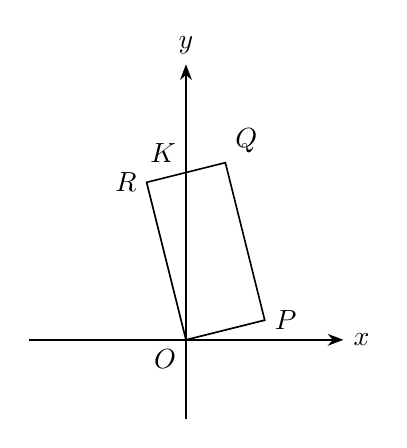
\begin{tikzpicture}[x=1cm,y=1cm,line width=.6pt,font=\normalsize,>=Stealth]
\coordinate (OL_O) at (0,0);
\coordinate (OL_P) at (1,0.25);
\coordinate (OL_Q) at (0.5,2.25);
\coordinate (OL_R) at (-0.5,2);
\coordinate (OL_K) at (0,2.125);
\draw[->] (-2,0)--(2,0) node[right] {$x$};
\draw[->] (0,-1)--(0,3.5) node[above] {$y$};
\draw (OL_O)--(OL_P)--(OL_Q)--(OL_R)--cycle;
\node[below left] at (OL_O) {$O$};
\node[right] at (OL_P) {$P$};
\node[above right] at (OL_Q) {$Q$};
\node[left] at (OL_R) {$R$};
\node[above left] at (OL_K) {$K$};
\end{tikzpicture}\hspace{8mm}%
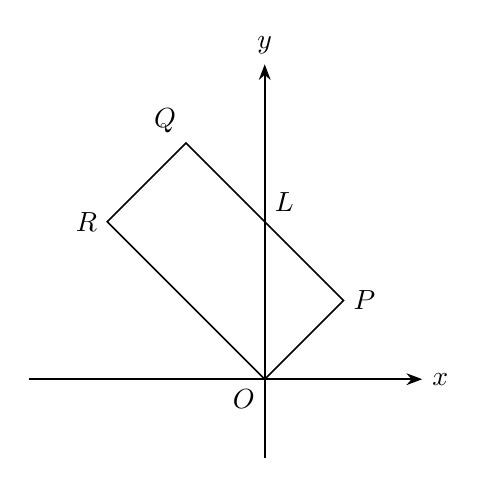
\begin{tikzpicture}[x=1cm,y=1cm,line width=.6pt,font=\normalsize,>=Stealth]
\coordinate (OR_O) at (0,0);
\coordinate (OR_P) at (1,1);
\coordinate (OR_Q) at (-1,3);
\coordinate (OR_R) at (-2,2);
\coordinate (OR_L) at (0,2);
\draw[->] (-3,0)--(2,0) node[right] {$x$};
\draw[->] (0,-1)--(0,4) node[above] {$y$};
\draw (OR_O)--(OR_P)--(OR_Q)--(OR_R)--cycle;
\node[below left] at (OR_O) {$O$};
\node[right] at (OR_P) {$P$};
\node[above left] at (OR_Q) {$Q$};
\node[left] at (OR_R) {$R$};
\node[above right] at (OR_L) {$L$};
\end{tikzpicture}
